% !TeX root = ../../../../01_git-vorgehensmodelle.tex

\subsection{Trunk-based Development}
\label{sec:workflows:trunk} 

Trunk-basierte Entwicklung, auch \emph{Trunk-based Development} (TBD) genannt, ist ein Vorgehensmodell, welches zum Ziel hat, die Schaffung von langfristigen Zweigen zu verhindern~\cite{trunkbased6}.

Es ist möglich, die Änderungen unmittelbar in den Master-Branch, auch \emph{Trunk} genannt, zu integrieren~\cite{trunkbased2}. Features oder Fehlerkorrekturen werden nicht in separaten Branches entwickelt, welche später mit \texttt{master} zusammengeführt werden~\cite{trunkbased2}. Vielmehr erfolgt die Integration sämtlicher Codeänderungen der Entwickler:innen direkt in einem gemeinsamen Hauptentwicklungszweig, der als zentrale Arbeitsgrundlage dient und sich zu jeder Zeit in einem produktionsreifen Zustand befinden soll~\cite{trunkbased1}.

Um zu erreichen, dass sich der Master-Branch in einem produktionsreifen Zustand befindet, sollen die Entwickler:innen ihre jeweiligen Änderungen häufig integrieren~\cite{trunkbased2}. Sämtliche Änderungen werden mindestens einmal am Tag wieder in den Hauptentwicklungszweig integriert, unabhängig davon, ob Feature\hyp Änderungen oder Erweiterungen bereits abgeschlossen sind oder nicht~\cite{trunkbased3}. Die Nutzung von Branches ist dann möglich, wenn es sich dabei um kurzlebige Branches handelt, die nach kurzer Zeit wieder im Trunk zusammengeführt werden~\cite{trunkbased7}, wie auch in \autoref{fig:trunk:TBD} dargestellt wurde. Dort wird veranschaulicht, dass Entwickler:innen sowohl direkt auf dem Trunk\hyp Branch arbeiten, als auch auf kurzlebigen Branches, welche mit dem Trunk zusammengeführt werden.


\begin{figure}
    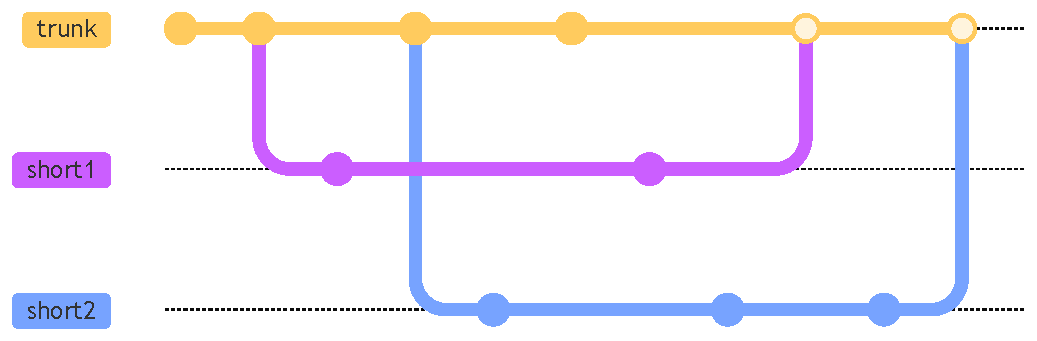
\includegraphics[width=0.45\textwidth]{src/assets/diagrams/trunk/trunk.pdf}
    \caption{Trunk-based Development: Trunk und zwei kurzlebige Branches (\texttt{short1} und \texttt{short2})}
    \label{fig:trunk:TBD}
    \Description{Git-Graph für Trunk-based Development mit einem Trunk und zwei kurzlebigen Branches}
\end{figure}

\subsubsection{CI/CD im Zusammenhang mit TBD}
\label{trunk:cicd}

Die Begriffe \emph{Continuous Integration} (CI) und \emph{Continuous Deployment / Delivery} (CD) werden häufig im Zusammenhang mit TBD genannt~\cite{trunkbased1,trunkbased2,trunkbased3}. Für eine ausführliche Definition kann unter \cite{trunkbased_cicd1} eingesehen werden.

Durch das regelmäßige Zusammenführen von Änderungen direkt in den Hauptentwicklungszweig können Zusammenführungs- und Integrationsphasen optimiert werden. Diese Vorgehensweise trägt dazu bei, die Ziele von CI/CD zu erreichen und verbessert die Softwarebereitstellung sowie die organisatorische Effizienz des Teams~\cite{trunkbased4}. Es wird sichergestellt, dass der Code zu jeder Zeit bereit für das Deployment ist, wodurch Continuous Delivery leichter umgesetzt werden kann~\cite{trunkbased5} und die Entwickler:innen dazu motiviert ihre Änderungen durch Tests abzusichern~\cite{trunkbased2}.

Durch Continuous Integration kann der Code automatisiert getestet und überwacht werden. Bei der Zusammenführung von neuem Code in den Trunk werden Integration und Codeabdeckung automatisch getestet, um stets die Qualität des Codes zu überprüfen~\cite{trunkbased4}.

\subsubsection{Verwendung von Feature Flags}
\label{trunk:ff}

Sogenannte \emph{Feature Flags} ermöglichen Entwickler:innen, bestimmte Abschnitte und Funktionen ihres Codes auszuschalten und sie zu einem späteren Zeitpunkt, nach vollständiger Entwicklung und Testung, wieder zu aktivieren~\cite{trunkbased_featureflag2}. Es handelt sich um eine Arbeitsweise, bei der Änderungen hinter einer \enquote{Flagge} in den Code integriert werden, um sie später wieder zu aktivieren oder sie auf kontrollierte Weise zu verbergen und zu entfernen. Daher erweisen sich Feature Flags für TBD als vorteilhaft, da Änderungen, die noch nicht für die Produktion bereit sind, exkludiert werden können, obwohl sie bereits im Code integriert sind~\cite{trunkbased_featureflag1}. Das hilft dabei den produktionsreifen Zustand beizubehalten, auch wenn beispielsweise bestimmte Features noch nicht vollständig funktionieren.

In \autoref{code:trunk:featureflag} wird eine  einfache Feature\hyp Flag\hyp Implementierung in JavaScript gezeigt. Dabei hängt das Verhalten der Funktion \texttt{feature} von der Variable \texttt{featureFlagAn} ab. Wenn man \texttt{featureFlagAn} auf \texttt{true} setzt, wird \texttt{Das Feature ist an} ausgegeben, andernfalls wird ein Standardverhalten ausgeführt.

\begin{listing}
    \inputminted[breaklines]{js}{src/assets/code/trunk/featureflags.js}
    \caption{Erstellung von Feature\hyp Flags}
    \label{code:trunk:featureflag}
\end{listing}  

\subsubsection{Vor- und Nachteile von TBD}
\label{trunk:vn}

So wie jedes andere Vorgehensmodell hat auch TBD seine Vor- und Nachteile, die in diesem Abschnitt kurz erläutert werden.

Einer der Hauptvorteile von TBD besteht in der reduzierten Komplexität des Merge\hyp Prozesses~\cite{trunkbased2}. TBD trägt dazu bei, die sogenannte \emph{Merge\hyp Hell} zu vermeiden~\cite{trunkbased2}, welches ein Problem in der Softwareentwicklung beschreibt, bei dem das Zusammenführen von zahlreichen Änderungen und Branches verschiedene Konflikte und Fehler verursachen kann~\cite{trunkbased8}. Eine Lösung besteht in der Verwendung von TBD, da dadurch weniger Konflikte beim Merge entstehen~\cite{trunkbased1}.

Ein weiterer Vorteil von TBD liegt in der schnellen Bereitstellung des Codes~\cite{trunkbased8}. Daraus folgt eine Verkürzung des \emph{Feedback\hyp Loops}~\cite{trunkbased2}, da der Trunk stets produktionsreif sein sollte~\cite{trunkbased1} und daher ein frühes Feedback der Kund:innen gewährleistet wird~\cite{trunkbased2}.

Ein möglicher Nachteil von TBD besteht darin, dass die Stabilität des Hauptentwicklungszweigs gefährdet werden kann, bspw. wenn keine ausreichende Testabdeckung vorhanden ist~\cite{trunkbased1}.

Es könnten Probleme entstehen, wenn die Entwickler:innen ihre Änderungen nicht regelmäßig integrieren und diese nicht gründlich testen~\cite{trunkbased1}. 
Die Entwickler:innen müssen es daher schaffen, kleine und gut getestete Änderungen vorzunehmen.

\subsubsection{Verwendungszwecke}

Die Anwendung von Trunk-based Development kann in unterschiedlichen Szenarien erfolgen. TBD ist vorteilhaft bei Projekten mit hoher Entwicklungsgeschwindigkeit, da Änderungen klein gehalten und zügig in den Hauptentwicklungszweig integriert werden können~\cite{trunkbased1}.

Des Weiteren eignet sich TBD besonders zu Beginn eines Projekts, insbesondere wenn es sich bei dem Ziel um ein \emph{Minimal Viable Product} (MVP) handelt. Da Pull Requests nicht erforderlich sind, können die Entwickler:innen durch die Verwendung von TBD schnell neue Funktionen integrieren~\cite{trunkbased6}.

TBD kann außerdem für Projekte mit hohen Qualitätsansprüchen sinnvoll sein, da sich der Hauptentwicklungszweig dauerhaft in einem produktionsreifen Zustand befinden muss. Dadurch wird sichergestellt, dass die Qualität und Integrität des Codes dauerhaft hoch ist. Dies kann besonders für Projekte mit strengen Qualitätsstandards von großer Bedeutung sein~\cite{trunkbased1}.

Wenn ein Projekt eine schnelle Anpassung an Änderungen oder Kundenrückmeldungen erfordert, kann TBD eine flexible Entwicklung ermöglichen und damit eine gute Wahl darstellen~\cite{trunkbased6}. TBD eignet sich außerdem besonders gut für kleine Teams, da eine gute Kommunikation für diese Arbeitsweise notwendig ist~\cite{trunkbased1}.

Falls erfahrene Entwickler:innen zusammen arbeiten, wird die Verwendung von TBD empfohlen~\cite{Gadzinowski_trunk-based_nodate}. Wenn Arbeitsabläufe bereits etabliert sind, gibt TBD jeder Person die Möglichkeit der Selbstentfaltung, was vorteilhaft für die Entwicklung sein kann~\cite{Gadzinowski_trunk-based_nodate}.

\subsubsection{Best Practices}
\label{trunk:bestprac}

Um TBD möglichst effizient zu verwenden, sollten bestimmte Anforderungen im Projekt implementiert werden, um das Team darauf vorzubereiten~\cite{trunkbased_bestpractice1}. Dabei ist es wichtig die Verwendung von CI zu fördern (siehe \autoref{trunk:cicd}). Testprozesse sollten automatisiert werden, um die Prozessvalidierung zu beschleunigen und menschliche Fehler zu reduzieren~\cite{trunkbased_bestpractice1}. Es ist ratsam, ein robustes Test\hyp Framework zu verwenden, das sowohl Unit\hyp Tests für Codeabschnitte als auch Integrationstests für die Zusammenarbeit verschiedener Komponenten durchführt~\cite{trunkbased_bestpractice1}.

Mit Hilfe von Code\hyp Reviews können Fehler konkret identifiziert und das gemeinsame Verständnis des Codes gefördert werden~\cite{trunkbased_bestpractice1}. Wie bereits aufgeführt, kann es außerdem sinnvoll sein, Feature\hyp Flags zu verwenden, um einen produktionsreifen Zustand beizubehalten.

\subsubsection{Fazit}

Trunk\hyp based Development verzichtet auf langfristige Branches in der Entwicklung~\cite{trunkbased6}. Die Entwickler:innen können agil arbeiten und mit Hilfe von automatisierten Tests den Hauptentwicklungszweig zu jeder Zeit in einem produktionsreifen Zustand halten. Um TBD verwenden zu können, sollten bestimmte Anforderungen beachtet werden. Daher kann TBD nicht für jedes Projekt oder Team eingesetzt werden~\cite{Manturewicz_trunk-based_2023}.
